\section{Punto 1}
\begin{enumerate}[a)]
  \item \textit{Cómo se comportaría el algoritmo de Ordenamiento por Conteo si en el arreglo original se permiten elementos repetidos?}\\

  En la figura \todo{la figura} se plantea una traza de ejemplo de como funciona el algoritmo de ordenamiento por conteo con elementos repetidos

  \begin{figure}
    \centering
    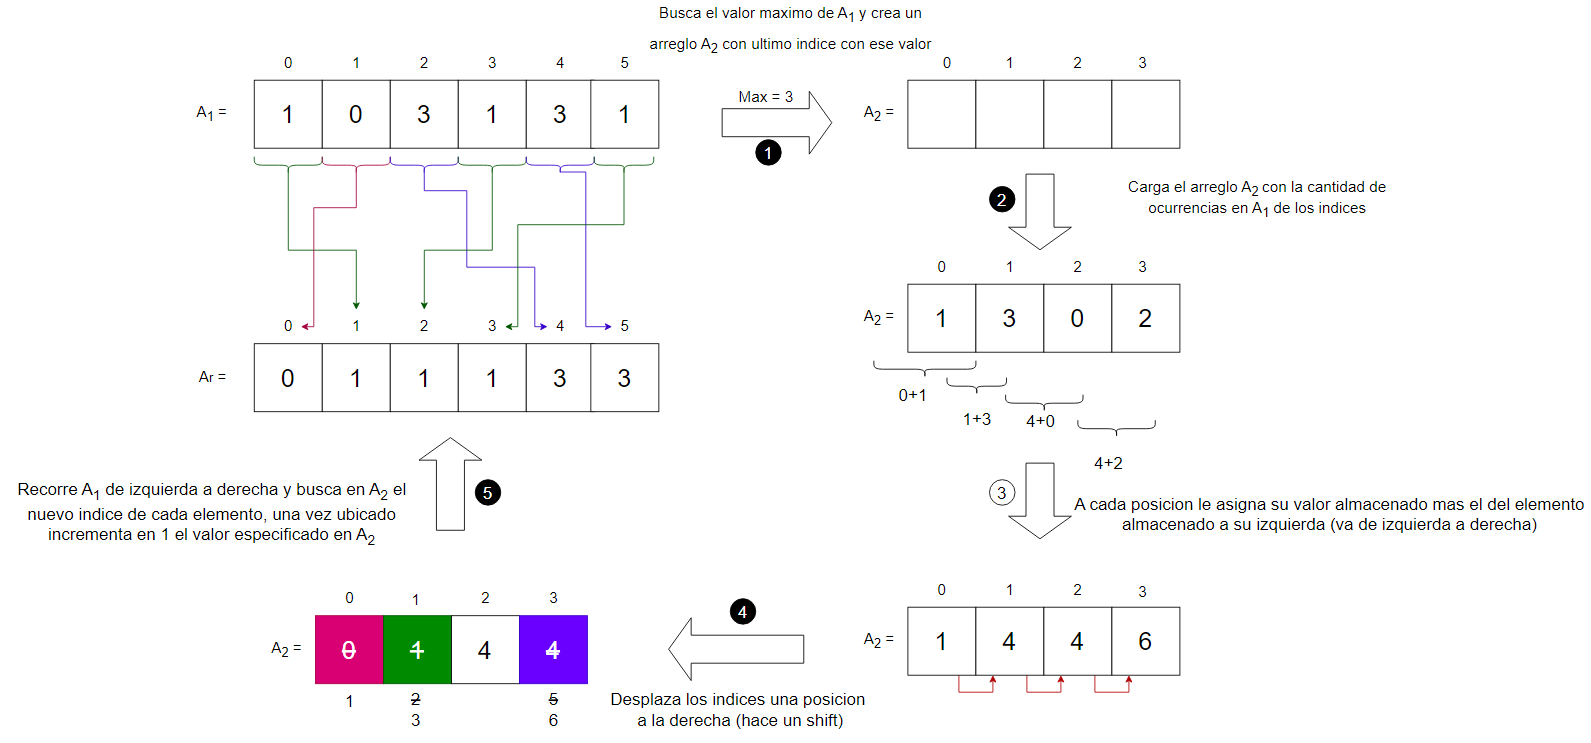
\includegraphics[width=\textwidth, scale=1]{Images/Punto1/Traza ordenamiento por conteo.png}
    \caption{Traza de algoritmo de ordenamiento por conteo}
    \label{fig:Traza ordenamiento por conteo}
  \end{figure}




  \item \textit{Modificar el algoritmo de Ordenamiento por Conteo para poder ordenar un arreglo de caracteres,
  de tal manera, que sean indistintas las letras mayúsculas y minúsculas, es decir que siempre se cumpla
  que:}\\
  $a<b$,\\
  $a<B$,\\
  $A<b$,\\
  $A<B$,\\
  \textit{En el arreglo resultante debe figurar cada letra en el mismo modo que en el arreglo original.
  }
\end{enumerate}